\section{Newton's method}

\subsection{Implementation}


We are going to use the class algorithm:


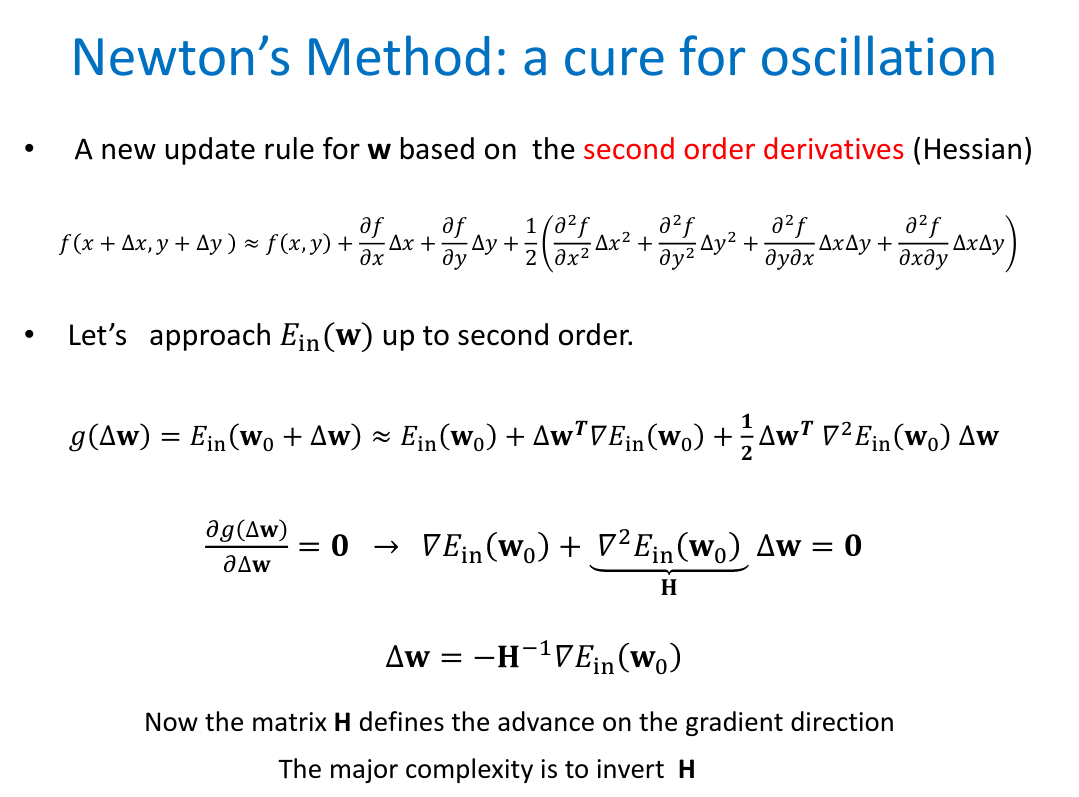
\includegraphics[width=\linewidth]{3_hessian_formula.png}

\subsubsection{Hessian matrix}

For function $f(x,y) = (x+2)^2 + 2(y-2)^2 + 2 \sin (2 \pi x) \sin (2 \pi y)$

\begin{equation*}
  \frac{\partial }{\partial x} f = 2 (x + 2) + 2 \sin (2 \pi y) \cos ( 2 \pi x) 2 \pi =  2 (x + 2) +  4 \pi \sin (2 \pi y) \cos ( 2 \pi x)   
\end{equation*}

\begin{equation*}
  \frac{\partial }{\partial y} f = 4 (y - 2) +  4 \pi \sin (2 \pi x) \cos ( 2 \pi y)   
\end{equation*}


\begin{equation*}
  \frac{\partial ^2 }{\partial y \partial x} f =  \frac{\partial ^2 }{\partial x \partial y } f =  8 \pi^2 \cos (2 \pi x) \cos ( 2 \pi y)   
\end{equation*}


\begin{equation*}
  \frac{\partial^2 }{\partial y^2} f = 4  -  8 \pi^2 \sin (2 \pi x) \sin ( 2 \pi y)   
\end{equation*}


\begin{equation*}
  \frac{\partial^2 }{\partial x^2} f = 2  -  8 \pi^2 \sin (2 \pi x) \sin ( 2 \pi y)   
\end{equation*}


\subsubsection{Implementation}

One implementation (really similar to the \texttt{gradient\_descent\_trace}

\begin{minted}{python}
def newton_trace(initial_point, fun, grad_fun, hessian, eta, max_iter):
    """ Newton method
    INPUT 
    - initial_point: 
    - f: differential function
    - grad_fun: Gradient
    - hessian: hessian
    - eta: learning rate
    - max_iter: number of iterations

    OUTPUT 
    w trace
    """

    w = initial_point
    w_list = [initial_point]
    iterations = 0

    while iterations < max_iter:
        w = w - eta *np.linalg.inv(hessian(w[0],w[1])).dot(grad_fun(w[0], w[1]))
        w_list.append(w)
        iterations += 1

    return np.array(w_list)

 \end{minted}


 The results after run are

 \begin{verbatim}
With eta = 0.01, 
coordenates (x,y)= (-0.9793498427941949, 0.9893767407575305), 
the number of iterations: 50 and the image is f(x,y) = 3.0671859515488302


With eta = 0.1, 
coordenates (x,y)=(-0.9463274028190676, 0.9717082373563009), 
the number of iterations: 50 and the image is f(x,y) = 3.1079767229661335
\end{verbatim}



 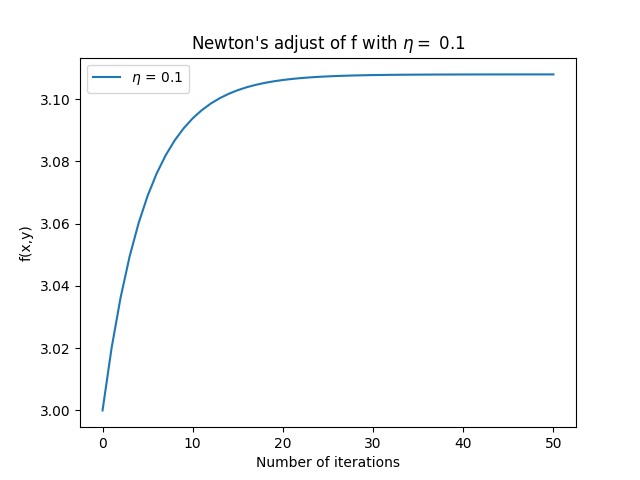
\includegraphics[width=\linewidth]{3_1_eta_01.png}
 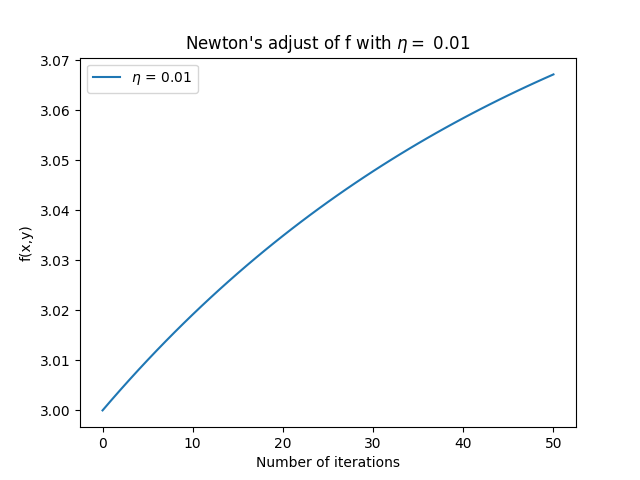
\includegraphics[width=\linewidth]{3_1_eta_001.png}
 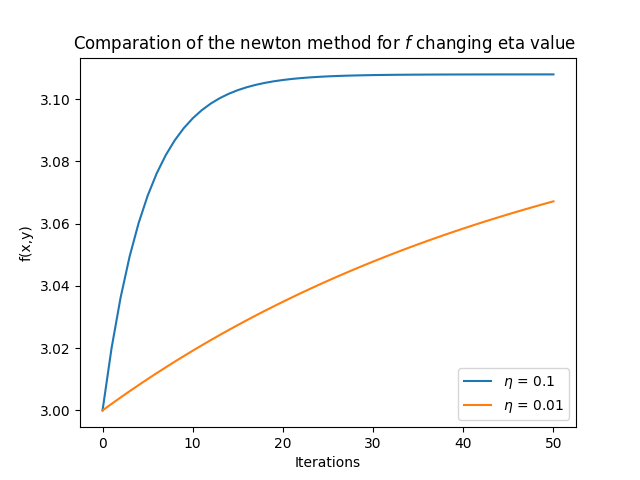
\includegraphics[width=\linewidth]{3_1_comparatives_etas.png}


 As we see this method does not minimize the function independently of the learning rate and even worse than the initial point. This is because this algorithm is sensible about where the gradient is zero.

 So in this case the algorithm get trapped in a saddle point.

 However if the function is convex it would be more precise even though the selection of the learning rating was bigger. 





\subsubsection{Different initial points }

\begin{center}
  \begin{tabular}{ |c|c|c| }
    \hline
    Initial point  & Final coordinates & Final value  \\ 
    \hline

    (-0.5 -0.5) & (-0.9463274,  0.97170824)  &  3.10798 \\
    (1, 1)    & [1.067, 0.911] &  11.345 \\
( 2.1, -2.1)   &  ( 3.261, -3.118)  & 78.711 \\
    (-3 , 3)  &  (-3.0536726 ,  3.02829176) &   3.108\\
(-2 , 2)  &  (-2,  2) &  0 \\
 
 \hline
\end{tabular}
\end{center}

If we compare with the gradient descendant's algorithm

\begin{center}
  \begin{tabular}{ |c|c|c| }
    \hline
    Initial point  & Final coordinates & Final value  \\ 
    \hline

    (-0.5 -0.5) &  (-0.793 -0.126) &   9.125 \\
(1 1) &  (0.677 1.29) &   6.437 \\
( 2.1 -2.1) &  ( 0.149 -0.096 ) &   12.491 \\
(-3  3) &  (-2.7315  2.713) &  -0.381 \\
(-2  2) &  (-2.  2.) &  0 \\
    
 
 \hline
\end{tabular}
\end{center}



So apart form the first one and the last point (which is a solution) the Newton's method is worse.

Let's see what is happening by plotting their traces. 

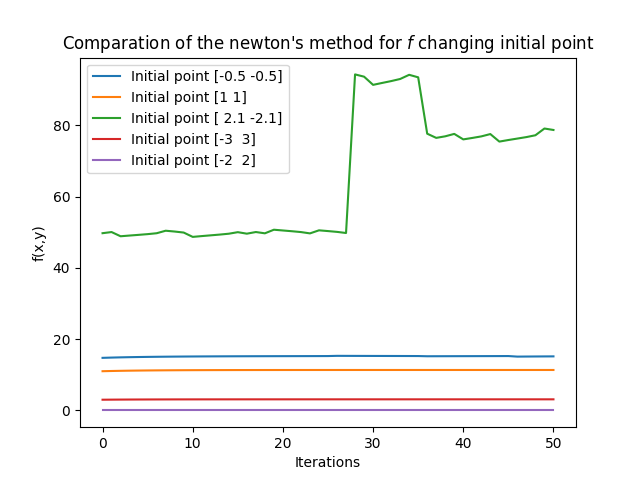
\includegraphics[width=\linewidth]{3_2_comparation_1.png}
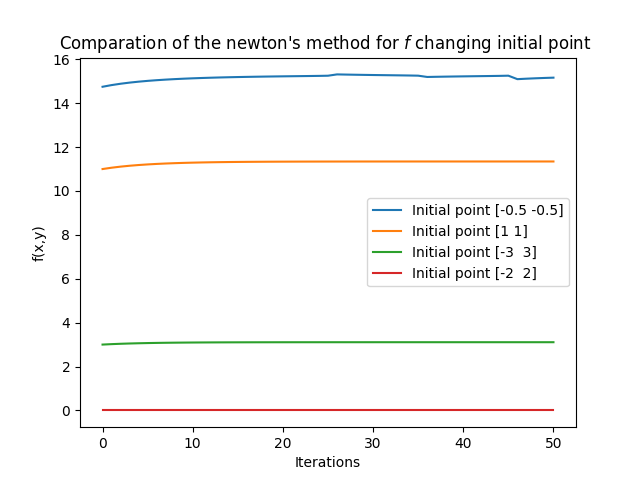
\includegraphics[width=\linewidth]{3_2_comparation_2.png}


Analysing the results we have observed that the points get easily trapped in a point, this may be because this algorithm is sensitive to the hessian.


If we compute these points' gradients and hessian we see that:

\begin{verbatim}

For (-0.38067878, -0.52778221)
	The gradient value is [ 1.64133153 -1.67813744]
	The inverse hessian is [[-0.00432244  0.01843361]
 [ 0.01843361 -0.00367461]]

For (1.06677195, 0.91078249)
	The gradient value is [ 0.03180694 -0.02149455]
	The inverse hessian is [[-0.00634209  0.01835718]
 [ 0.01835718 -0.00574093]]

For (3.26077803, -3.11750721)
	The gradient value is [ 11.09387996 -11.19723696]
	The inverse hessian is [[0.0182662  0.00126589]
 [0.00126589 0.0176255 ]]

For (-2.0, 2.0)
	The gradient value is [-6.15574622e-15  6.15574622e-15]
	The inverse hessian is [[-0.00064245  0.01268142]
 [ 0.01268142 -0.00032122]]

\end{verbatim}

As we thought the hessians of all these points are \textit{close} the null matrix.

\subsubsection{Conclusions}

This algorithm minimizes correctly the gradient but not the function. Therefore, if a function have saddle points this algorithm would not be as useful as the gradient descendent. Moreover, other problem is that the function should be twice differentiable. 
 